\documentclass[11pt]{article}
\usepackage[a4paper,margin=1in]{geometry}
\usepackage{amsmath,amssymb,amsthm,mathtools}
\usepackage{booktabs}
\usepackage{enumitem}
\usepackage{graphicx}
\usepackage{microtype}
\usepackage{hyperref}
\usepackage[nameinlink,capitalise]{cleveref}
\usepackage[numbers,sort&compress]{natbib}

\newtheorem{theorem}{Theorem}[section]
\newtheorem{proposition}[theorem]{Proposition}
\newtheorem{corollary}[theorem]{Corollary}
\theoremstyle{definition}
\newtheorem{definition}[theorem]{Definition}
\theoremstyle{remark}
\newtheorem{remark}[theorem]{Remark}
\newcommand{\norm}[1]{\left\lVert#1\right\rVert}
\newcommand{\tr}{\operatorname{tr}}

\title{Nonlinear Hybrid Horizon Budgets\\
\large Exact Propagation of Recursive Weak-Mode Quotient Losses}
\author{Liang Wang}
\date{July 2026}

\begin{document}
\maketitle

\begin{abstract}
RH-96 certifies the one-step energy loss from omitting weak projected-cross
directions, but more aggressive locally valid cutoffs still fail at the
endpoint.  We derive an exact horizon decomposition that does not linearize
the recursive Ritz map.

Let $F_t$ denote the full-width update, $A_t$ an adaptive update, $x$ the
source packet, and $J$ the endpoint tail.  Define the hybrid composition
\[
 H_j=F_N\circ\cdots\circ F_{j+1}\circ
 A_j\circ\cdots\circ A_1.
\]
Our nonlinear hybrid telescoping theorem is the identity
\[
 J(H_Nx)-J(H_0x)
 =\sum_{j=1}^N\bigl[J(H_jx)-J(H_{j-1}x)\bigr].
\]
It requires no linearity, differentiability, or common intermediate packet.
The triangle inequality gives an absolute propagated horizon budget.  If
$A_j=F_j$ except at sparse omission times, only those hybrid endpoints need
be replayed.

A 384-bit audit applies the identity to the three RH-96 cutoffs.  All ten
channel decompositions telescope and match the adaptive endpoint.  For the
primary $10^{-8}$ cutoff, the five omissions have worst absolute propagated
budget only $1.0035\times10^{-5}$ of the reference tail; the worst signed
endpoint shift is $7.06\times10^{-7}$.  The failing cutoffs are explained
quantitatively: their worst absolute budgets are $0.024921$ at $10^{-6}$ and
$0.014092$ at $10^{-4}$, each crossing the one-percent endpoint allowance in
exactly one channel.  Some hybrid contributions are negative, so future full
refresh can reverse a local quotient loss.

The endpoint threshold is therefore not mysterious: it is a propagated
budget threshold.  Hybrid replay is exact but a posteriori.  The next task is
a replay-free block propagation envelope.  No uniform repeated-block theorem,
Hilbert--Polya operator, zero identification, or Riemann Hypothesis result is
claimed.
\end{abstract}

\noindent\textbf{Keywords:} nonlinear telescoping; hybrid composition;
Duhamel principle; Ritz recursion; endpoint error budget; validated numerics.

\medskip
\noindent\textbf{MSC 2020:} 47A75; 39A30; 65F15; 65G20; 37C30.

\section{Introduction}

The gap-weighted theorem of RH-96 answers a local question: how much captured
energy can be lost when a weak complement direction is omitted
\citep{WangWeakMode2026}?  At relative cutoff $10^{-8}$, five such omissions
are harmless over the complete source-to-endpoint chain.  At cutoffs
$10^{-6}$ and $10^{-4}$, every local loss remains certified, yet one endpoint
fails.

A natural response is to postulate a linear recurrence
\[
 e_t\le\rho_te_{t-1}+\varepsilon_t.
\]
That form is useful eventually, but deriving a correct $\rho_t$ for a
recursive Ritz map is difficult.  The enrichment subspace depends
nonlinearly on the incoming packet through a projected cross SVD; different
width choices produce different packets, which then produce different future
subspaces.

This paper takes a more elementary route.  Replace one adaptive decision at a
time while replaying all later maps at full width.  The endpoint values of
these hybrid chains telescope exactly.  This is the discrete nonlinear
counterpart of a Duhamel or variation-of-constants decomposition
\citep{Deimling1985,HairerWanner1996}, but no derivative or tangent equation is
needed.

The decomposition has three advantages.
\begin{enumerate}[leftmargin=2em]
\item It attributes an exact endpoint contribution to each adaptive
decision, including its complete nonlinear future propagation.
\item It detects signed cancellation or reversal.
\item It turns the empirical endpoint frontier into a transparent absolute
budget.
\end{enumerate}
Its limitation is equally clear: it requires future replay.  RH-97 therefore
serves as an exact finite bridge between local quotient certificates and the
next desired analytic object, a reusable block propagation envelope.

\section{Nonlinear hybrid telescoping theorem}
\label{sec:theorem}

Let $X_0,\ldots,X_N$ be arbitrary sets.  For each time $t$, let
\[
 F_t,A_t:X_{t-1}\to X_t
\]
be full and adaptive maps.  Let $x\in X_0$ and let
$J:X_N\to\mathbb R$ be any endpoint functional.  No vector-space structure is
required.

\begin{definition}[Hybrid composition]
For $j=0,\ldots,N$, define
\begin{equation}
 H_j=
 F_N\circ\cdots\circ F_{j+1}\circ
 A_j\circ\cdots\circ A_1,
 \label{eq:hybrid}
\end{equation}
where $H_0=F_N\circ\cdots\circ F_1$ and
$H_N=A_N\circ\cdots\circ A_1$.
\end{definition}

\begin{theorem}[Nonlinear hybrid telescoping theorem]
\label{thm:hybrid}
For arbitrary maps and endpoint functional,
\begin{equation}
 J(H_Nx)-J(H_0x)
 =\sum_{j=1}^N\Delta_j,
 \qquad
 \Delta_j:=J(H_jx)-J(H_{j-1}x).
 \label{eq:telescoping}
\end{equation}
\end{theorem}

\begin{proof}
The right side is the telescoping sum of the scalar sequence
$J(H_0x),\ldots,J(H_Nx)$.  No relation between the intermediate states of two
different hybrids is needed.
\end{proof}

The simplicity of the proof is the point.  All nonlinear propagation is
contained inside the endpoint evaluation of $H_j$.

\begin{corollary}[Absolute propagated horizon budget]
\label{cor:absolute}
\begin{equation}
 \left|J(H_Nx)-J(H_0x)\right|
 \le\sum_{j=1}^N|\Delta_j|.
 \label{eq:absolute}
\end{equation}
\end{corollary}

\begin{corollary}[Sparse-decision reduction]
\label{cor:sparse}
Suppose $A_j=F_j$ outside an index set
$S=\{j_1<\cdots<j_q\}$.  Then $H_j=H_{j-1}$ for $j\notin S$, and
\begin{equation}
 J(H_Nx)-J(H_0x)
 =\sum_{\ell=1}^q
 \bigl[J(H_{j_\ell}x)-J(H_{j_\ell-1}x)\bigr].
 \label{eq:sparse}
\end{equation}
Thus only $q+1$ endpoint values are required.
\end{corollary}

\begin{remark}
The hybrid contribution $\Delta_j$ is not necessarily positive, even if the
adaptive one-step tail is larger than the full one-step tail.  Later nonlinear
full refreshes can contract, cancel, or reverse the injection.
\end{remark}

\section{Application to recursive Ritz refresh}
\label{sec:ritz}

For a fixed Gram sequence $G_1,\ldots,G_N$, let $F_t$ be the width-four
projected-cross Ritz refresh.  For a threshold $\tau$, let $A_t^\tau$ choose
the adaptive width of RH-96, between two and four.  Both maps act on
rank-$r$ packet projectors.  The endpoint functional is
\[
 J(V)=\mathcal E_{G_N}(V)
 =\tr G_N-\tr(V^*G_NV).
\]

At one omission time $j$, RH-96 supplies a local tail injection
\[
 \varepsilon_j
 =\mathcal E_{G_j}(A_j^\tau V_{j-1})
 -\mathcal E_{G_j}(F_jV_{j-1})\ge0.
\]
RH-97 instead measures
\[
 \Delta_j
 =J(H_jV_0)-J(H_{j-1}V_0),
\]
which includes all later full-width propagation.  The ratio
$\Delta_j/\varepsilon_j$ is a signed finite propagation multiplier.  It is a
diagnostic, not assumed a priori.

The absolute budget is normalized by the ambient leading-packet reference
tail at time $N$:
\begin{equation}
 B_\tau
 =\frac{\sum_{j\in S_\tau}|\Delta_j|}
 {\mathcal E_{G_N}(V_N^{\rm ref})}.
 \label{eq:budget}
\end{equation}
The inherited endpoint allowance is $B_\tau<0.01$.

\section{Validated experiment}
\label{sec:audit}

\subsection{Protocol}

We use the same ten channels, source seeds, rank clock, memory Gramians, and
endpoints as RH-94--RH-96 \citep{WangSourceSeed2026}.  For each threshold
$10^{-8},10^{-6},10^{-4}$:
\begin{enumerate}[leftmargin=2em]
\item run the adaptive chain and record its omission times;
\item run the full-width endpoint $H_0$;
\item after each omission, take the actual adaptive prefix packet and replay
all remaining updates at width four to obtain the next hybrid endpoint;
\item evaluate every endpoint tail as an exact-binary quadratic form in Arb at
384 bits \citep{Rump2010}.
\end{enumerate}
The interval sum of hybrid contributions is checked against the direct
adaptive-minus-full endpoint interval.  The last hybrid is also checked
against the adaptive endpoint.

\subsection{Primary five-omission budget}

All ten primary decompositions telescope, including the five channels with no
omission, where the budget is exactly zero.  The five nonzero contributions
occur at the same updates isolated in RH-95 and RH-96.

The worst absolute horizon budget is
\[
 B_{10^{-8}}\le1.00343\times10^{-5}.
\]
This is roughly three orders of magnitude below the one-percent allowance.
The worst signed endpoint shift is smaller still:
\[
 \frac{|J(H_Nx)-J(H_0x)|}{\mathcal E_{G_N}(V_N^{\rm ref})}
 \le7.06\times10^{-7}.
\]
Two of the five propagated contributions are negative and three are positive.
The largest absolute propagation multiplier is one; no primary local
injection is amplified at the endpoint.

\subsection{The failed thresholds}

\begin{table}[t]
\centering
\caption{Worst hybrid horizon budgets over ten channels.}
\label{tab:budgets}
\begin{tabular}{@{}lrrrr@{}}
\toprule
cutoff & omissions & absolute budget & signed shift & green channels\\
\midrule
$10^{-8}$ & 5  & 0.00001004 & 0.00000071 & 10\\
$10^{-6}$ & 11 & 0.02492070 & 0.02492070 & 9\\
$10^{-4}$ & 22 & 0.01409149 & 0.01409149 & 9\\
\bottomrule
\end{tabular}
\end{table}

\Cref{tab:budgets} explains the endpoint failures without appealing to a
heuristic accumulation story.  In the unique failing channel for each
aggressive cutoff, the propagated absolute budget crosses one percent.  The
signed shift is nearly the absolute sum there, so cancellation does not rescue
the endpoint.

Across all thresholds, some individual contributions are negative.  The
nonlinear future chain can improve the endpoint after a locally weaker choice.
This is why a product of positive scalar local losses would be an incomplete
description.

\begin{figure}[t]
\centering
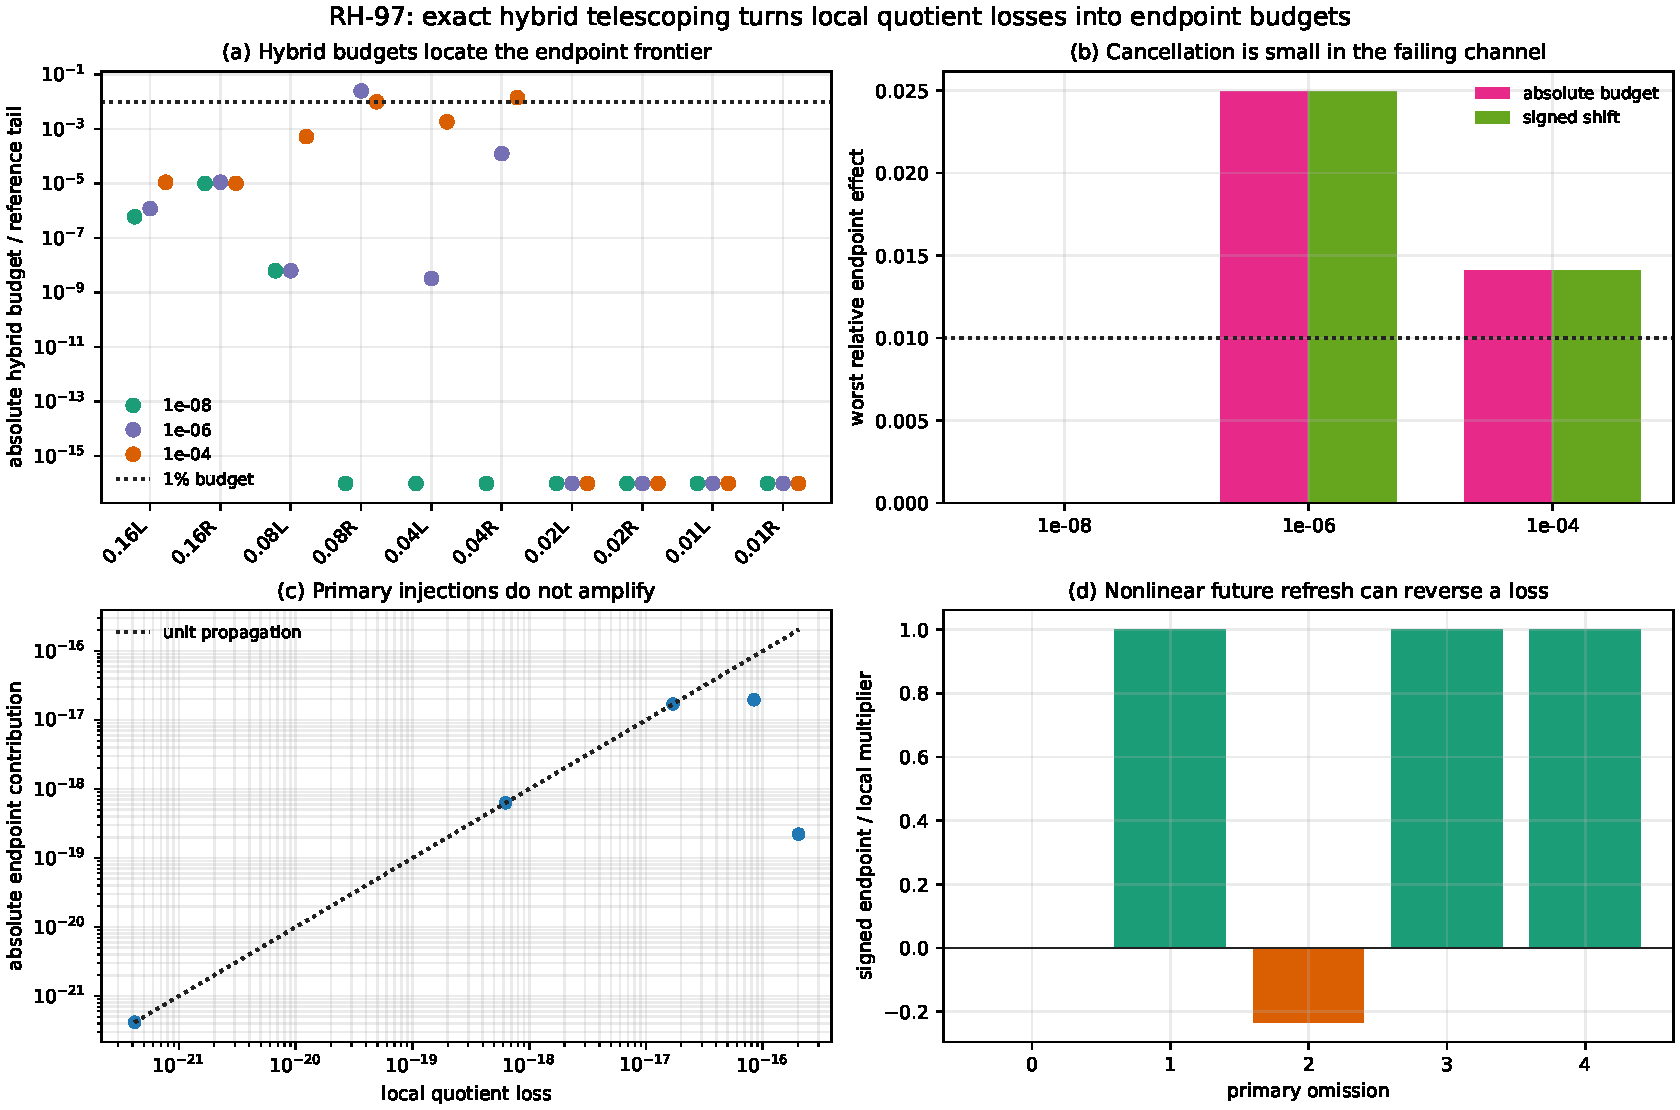
\includegraphics[width=\textwidth]{figures/nonlinear_hybrid_horizon_budget.pdf}
\caption{Exact nonlinear hybrid budgets.  The primary cutoff stays far below
one percent, while the two failed thresholds cross the inherited endpoint
allowance in exactly one channel.}
\label{fig:audit}
\end{figure}

\section{From hybrid replay to a block envelope}
\label{sec:next}

Hybrid replay solves the finite attribution problem exactly, but does not yet
give an analytic all-level theorem.  A reusable result would bound
$|\Delta_j|$ from information available near the injection time.  One target
is
\begin{equation}
 |\Delta_j|\le\Gamma_{j,b}\varepsilon_j,
 \label{eq:envelope}
\end{equation}
where $\Gamma_{j,b}$ is a propagation envelope for the future block $b$.

The audit suggests $\Gamma\le1$ for the tested omissions, but unit propagation
is not a formal consequence of Ritz monotonicity: two chains enter future
updates with different packets and different projected-cross spaces.  RH-98
should therefore either:
\begin{enumerate}[leftmargin=2em]
\item derive a sufficient compressed spectral condition implying
\eqref{eq:envelope}; or
\item construct a finite counterexample to unit propagation and identify the
weakest corrected envelope.
\end{enumerate}
A block envelope, combined with the local gap losses of RH-96, would produce a
replay-free horizon budget and prepare the route for repeated blocks or a
stopped exit clock.

\section{Block grouping and verification structure}
\label{sec:block}

The scalar hybrid sequence can be grouped at any chosen block boundaries.
Let
\[
 0=n_0<n_1<\cdots<n_B=N.
\]
Define the block increment
\[
 \Delta^{(b)}
 =J(H_{n_b}x)-J(H_{n_{b-1}}x).
\]
Then \cref{thm:hybrid} immediately gives
\begin{equation}
 J(H_Nx)-J(H_0x)=\sum_{b=1}^B\Delta^{(b)},\qquad
 |\Delta^{(b)}|
 \le\sum_{j=n_{b-1}+1}^{n_b}|\Delta_j|.
 \label{eq:block-budget}
\end{equation}
This grouped identity is exact even when several adaptive decisions inside a
block interact strongly.  It provides the correct target for a future block
envelope: one need not predict every individual signed contribution if a
single compressed certificate controls $|\Delta^{(b)}|$.

There are two distinct ways to use blocks.
\begin{enumerate}[leftmargin=2em]
\item \emph{Accounting blocks} merely aggregate already replayed hybrid
increments through \eqref{eq:block-budget}.
\item \emph{Predictive blocks} would replace those replays by a bound derived
from the block's initial packet, compressed spectra, and certified local
injections.
\end{enumerate}
RH-97 establishes the first exactly.  RH-98 must supply the second or show
why additional state variables are unavoidable.

\subsection{Sparse replay cost}

The naive hybrid family contains $N+1$ chains.  Sparse-decision reduction
changes this to $q+1$, where $q$ is the number of actual omissions.  In the
primary audit $q=5$ across all channels, rather than 120.  At the two larger
cutoffs, $q=11$ and $22$.  A hybrid starting at omission time $j$ replays only
the suffix $j+1,\ldots,N$, so the work is proportional to
\[
 \sum_{j\in S}(N-j),
\]
not $qN$ in every channel.  This remains a finite diagnostic cost, but it is
not a continuum complexity theorem.

\subsection{Interval closure}

Each hybrid packet is selected by floating-point SVD, QR, and small symmetric
eigensolves.  Once selected, its endpoint quadratic form is interpreted as an
exact binary input to Arb.  For interval endpoint values
$\boldsymbol J_j$, the audited contribution is the interval difference
\[
 \boldsymbol\Delta_j=\boldsymbol J_j-\boldsymbol J_{j-1}.
\]
The verification checks both
\[
 0\in
 \sum_j\boldsymbol\Delta_j-
 (\boldsymbol J_N-\boldsymbol J_0)
\]
and equality of the final hybrid with the directly computed adaptive
endpoint.  The absolute budget uses the largest absolute endpoint of each
$\boldsymbol\Delta_j$, so outward rounding cannot make a failing budget look
smaller.

This protocol validates the endpoint values of the concrete selected packet
chains.  It does not validate the discontinuous SVD branch choice against all
nearby real inputs; that stronger perturbation question belongs to the future
block envelope.

\section{Claim boundary}

The nonlinear hybrid telescoping theorem and absolute propagated horizon
budget are exact for arbitrary maps.  The numerical conclusions concern the
ten frozen packet chains.  We do not prove an a priori Ritz-refresh Lipschitz
law, a uniform block propagation envelope, repeated-horizon contraction,
Stage-A closure, a Hilbert--Polya operator, zeta-zero identification, or the
Riemann Hypothesis.

\section{Conclusion}

The local-to-global gap in adaptive Ritz enrichment can be closed exactly at
finite horizon by hybrid compositions.  Five primary omissions consume only
$10^{-5}$ of the reference tail, while the failed cutoffs consume 1.4--2.5\%.
The endpoint frontier is therefore a propagated budget frontier.

The remaining issue is not how to attribute loss, but how to predict its
future propagation without hybrid replay.  A compressed block envelope is
the next precise gate.

\bibliographystyle{plainnat}
\bibliography{references}

\end{document}
